\documentclass[dissertation]{softeng}

\usepackage{times}
\usepackage{outline}
\usepackage{ulem}
\usepackage{mdwlist}

%% XXX title needs work
\title{MoCaml: automatic dependency generation for OCaml}
\author{Mike McClurg}
\organisation{University of Oxford}
\college{Kellogg College}
\award{Software Engineering}

\date{\today}

\begin{document}

\maketitle

\begin{abstract}

  %% You should include a 100 to 200 word abstract.

  Object mocking is a technique to assist programmers in writing unit
  tests, by replacing hard-to-test dependencies with ``mock''
  implementations of those dependencies. A mock object allows the
  developer to set certain expectations about how the system under
  test will interact with the dependency, and then verify that these
  expectations hold true at the end of the test. While this technique
  was developed as a test design pattern for object oriented
  languages, it can also be useful for functional programming
  languages, especially for applications in which hard-to-test side
  effects can't easily be factored out of impure functions. This
  dissertation will explore the current state of the art tools and
  techniques for unit testing and mock object generation in object
  oriented languages. It will make the case that these techniques can
  be of use in functional programming languages, and it will describe
  the implementation and use of a new mocking library for the OCaml
  programming language.

  % ... Alas, functional languages are not immune to ...

\end{abstract}

\newpage

\begin{centering}

This thesis is dedicated to my wife, without whom I likely would never
have started writing.

\end{centering}

\newpage

\tableofcontents

%% Include chapters
\chapter{Introduction}
\label{introduction}

%% XXX consistent capitalisation of Mock Object and other Test Pattern names

This dissertation will explore the use of a unit testing technique
called the ``Mock Object Pattern'' in the strongly, statically typed
functional programming language OCaml. Mocking (or object mocking, as
it is more commonly known) is method of replacing hard-to-test
dependencies in object-oriented code with automatically generated
objects in order to make it easier to write unit tests. The technique
was first applied for use in Java, which is an object oriented
language with static types and run-time instrumentation facilities.

%% This disertation will describe the current state-of-the-art in unit
%% testing, specifically as it applies to functional programming
%% languages similar to OCaml (XXX just cover the thesis' organisation
%% here).

The dissertation is organised as follows. Chapter \ref{introduction},
Introduction, briefly describes the topic of software testing and
introduces the topic of Mock Objects. Chapter \ref{background},
Background, describes software testing in more detail, including
different levels of testing, common test design patterns, and tools
commonly used for testing. Chapter \ref{application}, Application,
describes the implementation of a tool, MoCaml, to assist OCaml
developers in automatically generating mock dependencies, and compares
tests written using this tool versus other similar tools. Chapter
\ref{reflection}, Reflection, describes the experience of writing
tests using MoCaml to write tests.

\section{Motivation of this dissertation}

%% We want to show why it is important to test software

%% Why is testing important? Include the statistic about how expensive
%% bugs are to fix after code has been shipped.

\subsection{Why write unit tests}

Automated testing is an important part of software development. At its
most basic, software testing is a means of demonstrating the quality
of software -- and the costs of poor quality in software can be
huge. In 2002, the US National Institute of Standards and Technology
estimated that poor software testing practices may cost the US between
\$22.2 and \$59.5 billion USD per year (not including the costs of
``mission critical'' software whose failure could lead to catastrophic
failure or loss of life). Furthermore, studies have shown that the
cost of fixing a software defect in production may be up to two orders
of magnitude greater than if the bug had been fixed in the development
phase. \cite{mcconnell:code} \cite{boehm:understanding} While this
``orders of magnitude'' statement has been part of the software
engineering lore since Boehm first made the observation in 1988, more
recent analysis \cite{boehm:software} \cite{bossavit:leprechauns}
indicates that the ratio of cost between fixing a bug in development
versus production may be closer to 1:5 rather than
1:100. Nevertheless, this is still a strong motivation to resolve
software defects as early as possible in the development cycle.



% testing versus static type checking



%% Much of the below is lifted from the proposal. I need to chop out
%% some stuff that's not necessary here, and beef up the parts that
%% are.

% types of tests. probably don't need this?

Software tests are typically grouped into three different levels:
system tests, component tests, and unit tests
\cite{ieee:glossary}. These categories represent a spectrum of
granularity. Systems tests represent the broadest granularity, and are
meant to test the entire system as a whole. On the other end of the
spectrum are unit tests, which test functionality at the finest level
of granularity: typically a method or function. Component tests sit
somewhere in between the two ends of the spectrum, and might test
interactions between modules or classes of an application, or perhaps
the interaction between distinct services of a larger
application. Some textbooks, particularly those describing Agile
software development practices, prefer the terms acceptance and
integration tests over system and component tests
\cite{freeman:growing} \cite{humble:continuous}. While these terms are
perhaps more descriptive of the objective of the different types of
tests, in this dissertation we will prefer to use the terms system and
component test, which better demonstrate {\em what} is being tested.

Recent trends in Agile development, such as continuous integration
\cite{humble:continuous} and test driven development \cite{beck:tdd},
have placed a greater emphasis on unit testing. Consequentially, many
tools and libraries have been developed to assist programmers in
writing these tests. Many of these libraries, such as JUnit
\cite{www:junit} for Java, NUnit \cite{www:nunit} for .NET, Test:Unit
\cite{www:ruby:unit} and RSpec \cite{www:rspec} for Ruby, and OUnit
\cite{www:ounit} for OCaml, follow the xUnit patterns of test
development described by Meszaros \cite{meszaros:xunit}. This family
of libraries typically provides a set of convenient assertion
functions to help the user write test cases, annotations to help
organise these test cases into larger test suites, and test harnesses
to handle test running and status reporting.

%\subsection{What are Mocks}
\subsection{Unit testing terms}

%% Describe xUnit pattern component names

%% XXX This might be a better fit for the Background section. Perhaps
%% we want a smaller introduction to Mocks in the Intro?

To understand mock objects, we should first familiarise ourselves with
the xUnit Pattern Language \cite{meszaros:xunit}. A pattern language
is a high-level, often visual, framework for describing patterns that
occur in software engineering. The xUnit Pattern Language has a
vocabulary that aids in describing the patterns that commonly occur
in unit testing. Primarily, it contains a vocabulary that covers most
aspects of software engineering and software testing. The following is
glossary of terms we will use in the following chapters.

\begin{description}

\item[System Under Test (SUT)] The part of the software that is being
  tested. Confusingly, this doesn't necessarily refer to the system as
  a whole, but rather the component of the system that is actually
  being tested. For instance, if we are testing a particular HTTP
  handler of a web application, the SUT is the HTTP handler itself,
  not the web application as a whole.

\item[Depended-On Component (DOC)] A component of the software which
  is a required dependency of the SUT. For instance, the HTTP handler
  we are testing may make a database query through an object
  relational mapper (ORM). In this case, the ORM is a DOC. A SUT may
  have more than one DOC.

\item[Dependency Injection (DI)] The act of configuring a SUT's
  dependencies, either at compile-time or run-time. A dependency which
  is configured at compile-time is often described as a ``hard-coded''
  dependency. Various dependency injection frameworks exist which
  provide facilities for configuring dependencies at run-time. For
  instance, a DI framework might instruct the ORM to map to a test
  database when a program is run in test mode, but would map to the
  real database when the program is run in production. This prevents
  the components of the software which interact with the database
  through the ORM from having to handle special-cases for testing
  purposes.\footnote{Dependency injection is not necessarily a part
    of the xUnit Pattern Language, but it is defined here because
    dependency injection plays an important role in the construction
    of tests that use the mocking technique.}

% p. 209
\item[Hard-to-Test Code] For many reasons, some software components
  will be hard to test. A component may depend on external data that
  isn't available at test time. A component may require certain
  specialised hardware to run which isn't available at test time. A
  component may be difficult to access programmatically (such as a GUI
  or web interface). Or the software may be written in a way that will
  make tests brittle and prone to breaking (such is the case with
  tightly coupled components). Refactoring may help make tightly
  coupled code easier to test, but some components may just be
  intrinsically hard to test.

% p. 59
\item[Test fixture] Tests often require certain infrastructure to be
  set up prior to a test run. A test database may need to be
  instantiated, or the program may need to be guided into a certain
  state before a particular test is run. The component which handles
  setting up this infrastructure is known as the test fixture
  (sometimes referred to as a test harness). Test fixtures often use
  a form of dependency injection to set up tests.

%% is this definition necessary?
%% \item[Test suite] A collection of tests which are meant to be run
%%   together.

%% Are we spilling the beans to early here?
\item[Test double] It may be impossible to test the SUT because it
  contains a DOC which is hard-to-test. In this case, the test double
  pattern can be used. A test double is a replacement for a
  hart-to-test DOC which makes it possible to test the SUT. xUnit
  defines the following test doubles: Test Stub, Test Spy, Mock
  Object, and Fake Object. In addition to these types of double, test
  doubles may either be configurable at run time, or have their
  configuration hard-coded. Test doubles will be further discussed in
  section \ref{testdoubles}, where we will discuss the mock pattern in
  much greater depth.

\end{description}

xUnit Test Patterns also defines the four phases of the testing life cycle:

\begin{enumerate}

\item \textbf{Setup} Initialise the required state so that the unit
  test is ready to be run. Depending on the test case, this may
  involve starting an http server, initiating a connection to a
  database and loading test data, or simply creating a test double and
  injecting it into the SUT. The point here is to provide context for
  the SUT to be executed.

\item \textbf{Exercise} This step simply executes the SUT in question
  within the context provided by the setup phase.

\item \textbf{Verify} Determine whether the test passed or failed by
  comparing the results of the execution phase to the expected
  results. This is typically accomplished by calling an \code{assert}
  function provided by the unit test framework being used, although it
  could be a more complext step such as verifying new database
  records, or calling a mock object's verification
  method.%% \footnote{Mocks will be covered in greater detail in section
    %% \ref{testdoubles:mocks}}

\item \textbf{Teardown} Cleanup after the test has finished. This
  involves undoing anything that was done in the setup phase, and
  perhas cleaning up any unwanted output generated by the SUT in the
  exercise phase, such as log files, etc.

\end{enumerate}

\section{Test doubles and the mock pattern}

For various reasons, some code is just hard to test. Often this
manifests itself in the form of hard-to-test dependencies of the
SUT. Examples of these DOCs may include queries to databases,
side-effecting code that is infeasible to run in a test environment,
or, as in the case of Test-Driven Development \cite{beck:tdd}, we are
testing a SUT which has a DOC that has not yet been fully implemented.

A SUT may be hard to test not only because of a hard-to-test DOC, but
because it is difficult to verify that the SUT has interacted with the
DOC in an appropriate way. For instance, we may want to test that the
SUT has sanitised its inputs before calling out to the ORM, but to do
so would require intercepting calls to the ORM, or modifying the ORM
specifically for the test case. The solution to this type of testing
problem is known as Behaviour Verification \cite{meszaros:xunit}.

The Test Double Pattern is a solution to the hard-to-test DOC
problem. A test double is an implementation of the DOC's interface
which can be used as a drop-in replacement for the DOC, thereby making
the SUT easier to test. Test doubles come in five flavours: Dummy
Objects, Test Stubs, Test Spies, Mock Objects, and Fake Objects. While
each of these types of test double can be used in place of a
hard-to-test DOC, each has a specific purpose that makes it better
suited for particular applications.

A Mock Object has unique capabilities that distinguish it from the
other test double patterns. A Mock Object implementes the interface
which we wish to replace, but allows the programmer to specify the
expected behaviour of the Mock during the test. These expectations may
specify both the expected inputs to a mocked method, as well as its
expected outputs. Mock Objects provide a verification method which
allows the test case to verify that the SUT interacted with the Mock
Object in the expected way. Mock Objects are also typically
automatically generated by the testing framework, and therefore are
considered to be dynamically configured test doubles. Because of these
properties, Mock Objects are very well suited for performing Behaviour
Verification.

\section{Current implementations of the Mock Object Pattern}

As implied by its name, the Mock Object pattern is a technique that
originated from the Object Oriented programming language
community. One of the first tools implemented to assist programmers in
writing Mock Objects was JMock \cite{www:jmock} for the Java
programming language. Mocking frameworks for other Object Oriented
languages exist as well, such as Moq \cite{www:moq} for C\# and .NET,
and RSpec \cite{www:rspec} for Ruby. These mocking frameworks each
support the automatic generation of mock implementations of objects
through the use of run-time reflection and code generation.

%% XXX need to double check the implemenetation of these libraries!

Reflection is a language feature which allows programs to perform
introspection at run time. In the case of mocking frameworks,
reflection is used to inspect a given class type (in Java's JMock and
.NET's Moq) or object (in the case of Ruby's RSpec) and generate an
object which implements the same interface as the orignal class type
or object. The framework provides functions for overriding the methods
of this generated object with user-provided expectations. The new
object can be used in place of the DOC in the SUT, and after the test
has executed, the mock's expectations can be verified.

Currently there is no implemetation of a dynaamically configurable
mock framework for OCaml that automatically generates mock
implementations of interfaces. The closest OCaml library for
implementing the Mock Object pattern is Xavier Clerc's Kaputt unit
testing tool \cite{www:kaputt}, which provides function combinators
for assisting programmers in writing hard-coded mock implementations
of functions. Compared to the dynamically configurable mocks generated
by the likes of JMock and RSpec, this is quite
cumbersome. Furthermore, the library only provides facilities for
mocking individual functions, meaning that if the user wants to write
a mock implementation of an entire module or object, then the user
must implement the entire interface manually, rather than just
providing expectations for the few functions exercised by the test
case.

Although it has neither run-time reflection nor run-time code
generation\footnote{While OCaml has execellent code generation
  facilities in the form of the \code{compiler-libs} library, it
  cannot generate at run-time code which could be executed by the same
  run-time environment.} capabilities, OCaml still has the potential
to host a dynamically configurable mocking framework, which could
fully implement a mock of a given interface and allow a programmer to
provide verifiable expectations for that mock. Among its many
benefits, OCaml has two important features we need: a strong, static
type system, and a powerful preprocessor and code generation facility
called camlp4 \cite{www:camlp4}. These two features will allow us to
write a fully-featured, dynamically configurable mocking framework for
OCaml.

\section{Objectives and expected contribution}

The objective of this dissertation is to create a dynamically
configurable mocking framework for OCaml, and to describe in detail
both its implementation and evaluate its use as a testing tool, in
comparison with mocking frameworks for other languages (both object
oriented and functional), and in comparison with other testing tools
for OCaml. In the background section, we will cover software testing
theory in more detail, and fully describe the Test Double patterns and
their use and implementation. In addition, we will discuss the OCaml
language, and explain how its features aid and hinder the
implementation of a mocking framework. Finally, we will discuss the
usefullness of the Mock Object pattern in a functional langauge
compared with its usefullness in an object oriented langauge.

%% Remaining TODO items:
%% - [X] make sure that code examples are finished (JMock needs work)
%% - [ ] adapt graphic descriptions of test patterns from xUnit book
%% - [ ] consider code examples of test pattersn besides mock objects
%% - [ ] consider changing the mock example to follow Freeman's turtle
%%       example

\chapter{Background}
\label{background}

In this section we will provide a brief tour of the OCaml programming
language, focusing especially on its powerful module system. The
chapter follows with a discussion of xUnit's Test Double patterns and
their implementation in OCaml and Java. The chapter concludes with a
summary of the current state-of-the-art testing tools for functional
languages such as OCaml and Haskell.

\section{A brief tour of OCaml and its module system}
\label{ocaml}

%% Define commands to change settings for Java and for OCaml. Need to
%% play with these more. Found this example at:
%% https://tex.stackexchange.com/questions/10141/how-to-prevent-lstlisting-from-splitting-code-between-pages
\lstnewenvironment{ocaml}[1][]%
  {\minipage{\linewidth} 
    \lstset{
      basicstyle=\ttfamily\footnotesize,
      language=ML,
      morekeywords={function,module,match,try},
      aboveskip=-\baselineskip,
      #1}}
  {\endminipage}

\lstnewenvironment{haskell}[1][]%
  {\minipage{\linewidth} 
    \lstset{
      basicstyle=\ttfamily\footnotesize,
      language=Haskell,
      morekeywords={function,module,match,try},
      aboveskip=-\baselineskip,
      #1}}
  {\endminipage}

\lstnewenvironment{java}[1][]%
  {\minipage{\linewidth} 
    \lstset{
      basicstyle=\ttfamily\footnotesize,
      language=Java,
      aboveskip=-\baselineskip,
      #1}}
  {\endminipage}

%% https://tex.stackexchange.com/questions/106844/adding-words-to-lstlisting-for-python-langaue
%% in order to get multiple levels of keywords
\lstset{
  language=ML,
  morekeywords={function,module,match,try},
  % Fix top/bottom frame margin spacing:
  % https://tex.stackexchange.com/questions/31598/lstlisting-produces-empty-row-when-used-inside-a-tabular
  aboveskip=-\baselineskip,
  %% framextopmargin=0pt,
  %% framexbottommargin=10pt,
  %% belowskip=10pt,
}

%% Want to talk quickly about code (functions, types, type inference),
%% modules, functors, first class modules. Mention that OCaml has a class
%% language, but that idiomatic OCaml typically uses functions and
%% modules unless a particular algorithm or solution to a problem
%% warrants an object-oriented implemtation.

OCaml is a strongly, statically typed functional programming language
based on the ML family of languages. It may be interpreted in a
read-eval-print loop called the OCaml ``toplevel,'' or it may be
compiled to an OCaml specific bytecode language or to a native
executable. \cite{ocaml:spec} It has a very good generational garbage
collector tuned for sequential programs. \cite{ocaml:gc_tutorial}

What follows is a \textit{very} brief tour of the OCaml programming
language. This should hopefully be enough to allow the reader to
follow along with the coding examples later in this chapter and the
next. For more assistance with OCaml, the reader is directed to the
OCaml Language Specification \cite{ocaml:spec}, and Real World OCaml
\cite{rwo}\footnote{Real World OCaml is available for free online:
  \url{https://realworldocaml.org}}

\subsection{OCaml basics: values, functions, and types}

\subsubsection{Values}

In OCaml, values are assigned to variables using the \code{let}
keyword.

\begin{lstlisting}
(* This is a comment *)
let num = 42
let str = "hello world"
let list = [1;2;3;4]
let tuple = (1,2)
\end{lstlisting}

Variables in OCaml are immutable, unless they are specially defined as
references, or mutable fields of a record type.

\begin{lstlisting}
let num = ref 42
Printf.printf "num was %d\n" !num
num := 24
Printf.printf "num is now %d\n" !num
\end{lstlisting}

\subsubsection{Functions}

Functions are created with the keywords \code{fun} or \code{function},
and assigned names using \code{let}, just like other values. Functions
defined using the \code{function} keyword can only take one argument,
but that argument can be pattern-matched.

\begin{lstlisting}
let f = fun a b -> a + b
let g = function
        | [] -> true
        | _  -> false
\end{lstlisting}

Functions can also be created using a shorthand \code{let} syntax. The
function \code{f} below is equivalent to the function \code{f} above.

\begin{lstlisting}
let f a b = a + b
\end{lstlisting}

Because functions are first-class values just like \code{int}s and
\code{string}s, we can pass them to other functions. For instance, the
function \code{List.map} takes a function \code{f} and a list
\code{ls}, and returns a new list containing the result of applying
\code{f} to each element of \code{ls}.

\begin{lstlisting}
let f x = x + 1
let ls = [1;2;3;4]
List.map f ls         (* returns the value [2;3;4;5] *)
\end{lstlisting}

\subsubsection{Types}

OCaml is a strongly, statically typed language. The compiler will
infer the type of values, and will return an error if a type
constraint is violated. For instance, the following function \code{f}
has type \code{int -> int -> int}, meaning that it takes two values of
type \code{int} and returns a value of type \code{int}. If a
\code{string} or \code{float} are passed to this function, a
compilation error is thrown.

\begin{lstlisting}
let f a b = a + b     (* has type int -> int -> int *)
f 40 2                (* this type-checks *)
f "4" "2"             (* this fails to type-check *)
f 41.8 0.2            (* this also fails to type-check *)
\end{lstlisting}

OCaml allows the user to define complex types.

\begin{lstlisting}
(* Tuples *)
type position = int * int

(* Variant types *)
type colours =
  | Red of int
  | Green of int
  | Blue of int

(* Record types *)
type book = {
  author : string;
  title  : string;
  mutable inventory : int;
}
\end{lstlisting}

%% type variables

Polymorphism in OCaml data types is expressed with type variables. In
the following example, \code{'a} is a type variable which can
represent any type, making \code{tree} a generic data type.

\begin{lstlisting}
type 'a tree =
  | Leaf of 'a
  | Node of 'a tree * 'a tree
\end{lstlisting}

\subsubsection{Polymorphic variants}

OCaml has a feature called \emph{polymorphic variants}. These are
similar to atoms or symbols in languages like Erlang or
Scheme. Polymorphic variants are distinguished from regular variants
by the backtick (\code{`}) preceding the label. Unlike regular
variants, polymorphic variants do not need to be capitalised, but this
is still common practice. A common use of polymorphic variants is to
encode inputs or outputs of functions; for instance, the below
function uses polymorphic variants for encoding success and failure
cases.

\begin{lstlisting}
let f = function
  | `String v ->
    Printf.printf "Got a string: %s\n" v;
     `Success
  | `Int v    ->
    Printf.printf "Got an int: %s\n" v;
    `Success
  | `Float _  ->
    print_endline "Wasn't expecting a float.";
    `Failure
\end{lstlisting}

Polymorphic variants can be used in the same way as regular variant
types, except that they don't need to be explicitly
declared. Furthermore, any polymorphic variant with the same name is
considered to be the same type (unlike regular variants, where
identically named constructors may be protected inside of different
modules, and therefore would be different types).

This gives rise to useful patterns in API development, such as
extensible API types. For instance, the Yojson library has an encoding
of standard JSON, as well as common, useful extensions to the JSON
spec. The standard JSON spec is encoded in \code{Yojson.Basic.json},
whereas the extensions to the standard are encoded in
\code{Yojson.Safe.json}. The \code{json} type in both modules uses
polymorphic variants to define the json grammar, and ``Basic'' JSON
can be easily upgraded to ``Safe'' JSON. A full treatment of this
library can be found in Chapter 15 of Real World OCaml \cite{rwo}.

\subsubsection{Pattern matching}

One of the most powerful features of languages like OCaml is pattern
matching. OCaml allows one to match over the structure of defined data
types. Pattern matching can be accomplished with the
\code{match value with | patt -> expr}
expression, or in functions created with the \code{function}
keyword. The following two functions are equivalent.

\begin{lstlisting}
let rec num_leaves_1 = function
  | Leaf _      -> 1
  | Node (l, r) ->
    (num_leaves l) + (num_leaves r)

let rec num_leaves_2 tr =
  match tr with
  | Leaf _      -> 1
  | Node (l, r) ->
    (num_leaves l) + (num_leaves r)
\end{lstlisting}

Note the use of the underscore (\code{_}) in the \code{Leaf}
pattern. In OCaml, underscore means ``match anything.'' It can also be
used in variable assignment, and is often used in module
initialisation code.

\subsubsection{Exceptions}

OCaml has exceptions that follow the usual ``try/catch''
pattern. OCaml exceptions have no ``finally'' clause, but this can be
implemented in a library using first-class
functions.\footnote{cf. \code{protect} and \code{protectx} in Jane
  Street's Core library:
  \url{https://ocaml.janestreet.com/ocaml-core/111.03.00/doc/core/#Exn}}
Exceptions are declared similarly to variant data types.

\begin{lstlisting}
exception Not_found
let rec find x = function
  | [] -> raise Not_found
  | (k,v)::ls -> if x = k
                 then v
                 else find x ls
\end{lstlisting}

As with variants, exceptions can also carry data:

\begin{lstlisting}
exception Failure of string
exception Error of [`Invalid_request of string | `Permissions]
raise (Error (`Invalid_request "foo"))
raise (Error `Permissions)
\end{lstlisting}

``try/catch'' blocks in OCaml are similar to those in other languages,
except OCaml pattern matches on the ``catch'' block using the
\code{with} keyword.

\begin{lstlisting}
try
  raise (Error (`Invalid_request "foo"))
with
  | Error `Permissions ->
    print_endline "Bad permissions"
  | Error (`Invalid_request req) ->
    Printf.printf "Invalid request: %s\n" req
\end{lstlisting}

\subsection{The OCaml module system}

\subsubsection{Modules, signatures, and compilation units}

A distinguishing feature of OCaml is its powerful module system. A
module in OCaml is the basic compilation unit. Each compiled file is
assigned its own module. For instance, the definitions inside a file
called \code{foo.ml} would be placed into a module \code{Foo}.

%% XXX not sure if we want these to come from separate files, or if we
%% want to put a border around them, or...
%% \lstinputlisting[
%%   caption=foo.ml,
%%   %frame=single,
%% ]{code/foo.ml}
\begin{lstlisting}
type t = int
let f a = a
\end{lstlisting}

From outside of this module, function \code{f} would be referenced as
\code{Foo.f}. Module \code{Foo} has the following type:

\begin{lstlisting}
type t = int
val f : 'a -> 'a
\end{lstlisting}

The types of modules can be restricted using \code{mli} files. When
an \code{mli} file exists with the same basename as an \code{ml} file,
the module type of the module created for that \code{ml} file is
restricted to that of the signature specified in the \code{mli}
file. For instance, if \code{foo.mli} is:

%\lstinputlisting[caption=foo.mli]{code/foo.mli}
\begin{lstlisting}
type t = int
val f : ’a -> ’a
\end{lstlisting}

then the resulting type of module \code{Foo} would be:

\begin{lstlisting}
type t
val f : t -> t
\end{lstlisting}

Notice that \code{type t} is now abstract (meaning that we can't know
its implementation outside of module \code{Foo}, and function \code{f}
is now restricted to have type \code{t -> t}, instead of the more
general \code{'a -> 'a}.

OCaml modules can also be defined independently of compilation
units.

\begin{lstlisting}
module Bar =
struct
  type t = int
  let g a = a + 1
  let h ls = List.map g ls
end
\end{lstlisting}

We can also create module type signatures, which can restrict the
resulting type of a module in the same way as an \code{mli} file.

\begin{lstlisting}
module type BAR =
sig
  type t
  val h : int list -> int list
end
\end{lstlisting}

We can limit the type of \code{module Bar} to the signature
\code{BAR} by restricting it:

\begin{lstlisting}
module Bar2 = (Bar : BAR)
\end{lstlisting}

We can also restrict the original definition of \code{module Bar}:

\begin{lstlisting}
module Bar1 : BAR =
struct
  type t = int
  let g a = a + 1
  let h ls = List.map g ls
end
\end{lstlisting}

Modules \code{Bar1} and \code{Bar2} are now restricted by the
signature \code{BAR}. The value \code{g} is now hidden, and
\code{type t} is now abstract.

\subsubsection{Functors}

In most languages, a module system is primarily meant to provide a
namespacing system or a way to refer to compilation units
(cf. Haskell's module system \cite{www:haskell:modules}, or Python's
module system \cite{www:python:modules}). OCaml, however, has a much
more powerful module system, including the ability to define
\textit{functors}.

A functor is a relation from modules to modules. A functor can take a
module as an argument, and use it to specialise another module. For
instance, here is an example adapted from the OCaml language
``Introduction to OCaml'' \cite{ocaml:spec} that creates a \code{Set}
functor.

\begin{lstlisting}
module type ORDERED_TYPE =
sig
  type t
  val compare: t -> t -> int
end

module Set =
  functor (Elt: ORDERED_TYPE) ->
    struct
      type element = Elt.t
      type set = element list
      let empty = []
      let add x s = ...
    end
\end{lstlisting}

\code{Set} is a functor that takes some module with same type
signature as \code{ORDERED_TYPE}, and returns a module which is
specialised with that element type. For instance, we may create a new
\code{StringSet} module using the \code{Set} functor and the
\code{String} module from the OCaml standard library.

\begin{lstlisting}
module StringSet = Set(String)

let set = StringSet.add "foo" StringSet.empty in
StringSet.mem "foo" set  (* => true *)
\end{lstlisting}

For brevity, OCaml supports and alternative syntax for functor
definition which is more concise. For instance, we could have defined
the \code{Set} functor as:
\code{module Set(Elt : ORDERED_TYPE) = struct ... end}.
This comes in handy when one is defining a functor which takes
multiple arguments:
\code{module F(A : X)(B : Y) = struct ... end} .

Functors are useful for creating generic data types, such as the
\code{Set} type we defined above. We will soon see that they can also
be useful for dependency injection.

\subsubsection{First-class modules}

OCaml 4.00 introduced the feature of \textit{first-class modules}. A
first-class module is analogous to a language having first-class
functions: a module in OCaml can be packaged into a value, passed to
functions, and returned from functions. First-class modules provide a
similar capability as functors do, but are much more
light-weight. Refactoring a module into a functor can be a significant
amount of work, but adding a module argument to a function is a much
simpler change.

\begin{lstlisting}
module type DATABASE = sig ... end

module Db = struct ... end

let f db =
  (* Turn a module value into a module *)
  let module Db = (val db : DATABASE) in
  ...

(* And convert a module into a value *)
let _ = f (module Db : DATABASE)
\end{lstlisting}

\subsection{The rest of OCaml}

%% Briefly mention OCaml's object system and class language, and point
%% the reader to books and web resources.

In addition to the module language described above, OCaml also has a
rich class language and object system. Object orientation is a useful
addition to OCaml, but most OCaml code in practice eschews the use of
objects and classes. This dissertation will ignore the object oriented
features of OCaml and instead focus on its functional core and module
system. Most of the literature regarding software testing assumes
an object oriented implementation language; this dissertations
contributions lie elsewhere.

This was a whirlwind tour of OCaml. It was meant to cover just enough
syntax to get the reader through the OCaml examples in the next
section, and to understand the implementation in the following
chapter. For more extensive coverage, please see the OCaml language
spec \cite{ocaml:spec}, and the excellent Real World OCaml book
\cite{rwo}.

\section{Test Double patterns in detail}
\label{testdoubles}

%% XXX consider citing Gibbons \cite{gibbons:patterns}

\begin{figure}
  \centering
  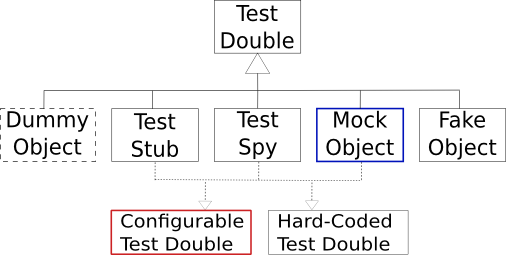
\includegraphics[scale=0.7]{img/test_double_taxonomy.png}
  \caption[Taxonomy of Test Double patterns]{Taxonomy of Test Double patterns\footnotemark}
  \label{fig:taxonomy}
\end{figure}
\footnotetext{Adapted from Meszaros \cite{meszaros:xunit}}

%%% (XXX) As figure \ref{fig:taxonomy} shows\dots

\begin{table}
  \centering
  \begin{tabular}{c|c|c|c|c|c}
    %% Header (in two parts for line-breaking)
    & Implements
    & Indirect
    & Indirect
    & Configurable
    & Behaviour
    \\
    & Interface
    & Inputs
    & Outputs
    &
    & Verification
    \\ \hline
    %% Rows
    \textit{Dummy} & No & No & No & No & No      \\ \hline
    Stub           & Yes & Yes & No & Yes & No   \\ \hline
    Fake           & Yes & No & No & N/A & No    \\ \hline
    Spy            & Yes & No & Yes & Yes & No   \\ \hline
    Mock           & Yes & Yes & Yes & Yes & Yes \\ \hline
  \end{tabular}
  \caption{Comparison of Test Double pattern features}
  \label{table:testdoubles}
\end{table}

Test Doubles allow developers to write tests that might have been
difficult or even impossible to write without a Test Double. As their
name suggests, Test Doubles are meant to stand in for a DOC of the
SUT. Their name is analogous to ``stunt doubles'' used in films to
stand in place for the main actor during dangerous scenes
\cite{meszaros:xunit}.

Meszaros describes three problematic scenarios for which Test Doubles
may be an appropriate solution.

\begin{description}

\item [Untested Requirement] A particular SUT may have a system
  requirement that needs to be exercised in a unit test, but testing
  this behaviour requires observing interactions between the SUT and
  one of its DOCs. If the DOC doesn't provide a mechanism for
  observing these inputs and outputs, a Test Double may be used in
  place of the DOC to observe the indirect inputs and outputs between
  the SUT and the DOC.

\item [Untested Code] A SUT may depend on a DOC which does not provide
  the test case enough control over its inputs to properly exercise
  the desired behaviour in the SUT. A Test Double for the DOC may be
  used in order to put the SUT into the state necessary to exercise
  this behaviour.

  Another instance of this issue occurs when the DOC has not been
  written yet, but a test for the SUT still needs to be written. This
  case often occurs in Test Driven Development (TDD) \cite{beck:tdd},
  where tests are usually written either before or during the
  development phase.

\item [Slow Test] Slow tests can be a major problem because they
  discourage the use of unit tests as part of the build process. A
  test may be slow because a particular DOC takes a long time to
  perform its task; perhaps it is performing a major calculation, or
  is downloading a file over a slow network connection. In this case,
  a Test Double may be used in place of the DOC in order to speed up
  the test cases which require this DOC.

\end{description}

\subsubsection{Indirect inputs and outputs}

Test Doubles have the benefit of being able to provide
\textit{indirect inputs} to the SUT, and to receive \textit{indirect
  outputs} from the SUT.

When exercising the SUT, we often need a way to control the
execution path of the SUT from the test case. In many cases, this is
not directly possible, because the SUT bases its execution path from
inputs received from one of its DOCs. These inputs are known as
\textit{indirect inputs}. In order to provide indirect inputs to the
SUT via the DOC, we can replace the DOC with a Test Double which
support indirect inputs (see table \ref{table:testdoubles}).

In order to verify that the SUT performed as expected during the test,
we may need to record the SUT's interactions with it's various
DOCs. These interactions are called \textit{indirect outputs} because
they are not directly visible from the test case itself. If a DOC does
not provide a way for the test case to read these indirect outputs in
a way that makes it possible to verify the correct behaviour of the
SUT, then a Test Double which supports indirect outputs may be used in
place of the DOC (see table \ref{table:testdoubles}).

\begin{figure}
  \centering
  
\includegraphics[scale=1.0]{img/indirect_inputs.png}
  \caption[Indirect Inputs]{Indirect inputs to a SUT\footnotemark}
  \label{fig:indirect_inputs}
\end{figure}
\footnotetext{Adapted from Meszaros \cite{meszaros:xunit}}

\begin{figure}
  \centering
  
\includegraphics[scale=1.0]{img/indirect_inputs.png}
  \caption[Indirect Outputs]{Indirect outputs from a SUT\footnotemark}
  \label{fig:indirect_outputs}
\end{figure}
\footnotetext{Adapted from Meszaros \cite{meszaros:xunit}}

\subsubsection{Common pitfalls of the Test Double patterns}

Using the Test Double patterns can make it easier to write unit tests,
but misuse of the patterns can cause problems. Because we are
replacing a DOC with a component that is custom-built for a particular
test case, we must be careful to avoid overly tight coupling between
the Test Double and the SUT. This can lead to \textit{Overspecified
  Tests}, which are a type of the \textit{Fragile Test} anti-pattern
\cite{meszaros:xunit}. A Fragile Test is one which may break due to
changes in the SUT which do not affect the behaviour being tested.

Another potential pitfall of misusing Test Doubles is the possibility
that the developer may accidentally replace the part of the SUT which
is being tested. This can be a severe problem, because tests for a
particular behaviour will show as passing, even though that behaviour
has never been exercised by the tests. Care should be taken when
writing tests to ensure that the test actually exercises the
behaviour under test.

\subsubsection{A note on terminology}

The xUnit Test Patterns book refers to the pattern as a \textit{Mock
  Object}. While OCaml does have object oriented features, we are
primarily concerned with mocking OCaml modules. In the rest of this
dissertation, we will use the term Mock Object when referring
specifically to the pattern described in the xUnit book, although we
mean to apply this pattern to OCaml's modules. When speaking of a
module that follows the Mock Object pattern, we may specifically refer
to this as a \textit{Mock Module}.

%% We will want to include diagrams relating all the test double
%% patterns, and describing them individually. The xunit web page has
%% many of these diagrams electronically, so we should use those where
%% we can, with proper attribution.

% http://xunitpatterns.com/Mocks,%20Fakes,%20Stubs%20and%20Dummies.html

%% XXX Should this go in a common definitions file? Probably...
\newcommand{\definition}[1]{\hangindent=1cm \textbf{#1}}

\subsection{Fake Object pattern}
\label{testdoubles:fake}

\definition{Fake Object} is a simpler version of the DOC which
performs the same function with less complexity.

A Fake Object is a simple replacement for a complex DOC. It does not
provide any test-specific features, such as the ability to deal with
indirect inputs or outputs. A Fake Object should be used when a SUT
has a complex DOC that makes it infeasible to run unit tests. For
instance, a web service DOC may be replaced by an object which returns
hard-coded results without the need to access the network. A database
may be replaced by a simpler data store such as a hash table or other
in-memory database.

%% TODO code example?

\subsection{Dummy Object pattern}
\label{testdoubles:dummy}

\definition{Dummy Object} is a special case of Test Stub which applies
to value types.

A \textit{Dummy Object} is a special case of a Stub Object. It is used
specifically when the SUT does not interact with the DOC at all during
the test, but a value for the DOC is still required in order to
initialise the SUT. For instance, the SUT may be a method of a class
which requires certain values to be constructed, but the SUT itself
doesn't make use of those values during the test. In a language with
nullable types, such as Java, a Dummy Object may simply be the
\code{null} value. In a language like OCaml, a Dummy Object may be a
value, such as a simple type constructor. A more complex type may have
a ``default'' or ``empty'' value that can be used. This is often the
case with record types, for which programmers often create an
``empty'' value which they can extend to create more complex
values. Many standard library containers have either an empty default
value, or a simple constructor, for instance \code{Set.empty} or the
value constructor \code{Buffer.create}, which takes a single integer
value.

%% A Dummy Object is used in place of a DOC when the SUT requires a
%% dependency for it's state, but the SUT doesn't use this dependency
%% during the test. It may be expensive to create a real instance of
%% the DOC, so a Dummy Object is created in its place. In languages
%% like Java, the \code{null} object may be used as a Dummy
%% Object. (What could we use in OCaml? Perhaps refactor so that the
%% DOC is an option type? OCaml types are often less complex than Java
%% objects, so we may have a simple constructor we can use instead of
%% null. A pattern we often use w.r.t. record types is to construct an
%% ``empty'' value of that type for later extension, so we could reuse
%% this value for testing purposes. Other than that, perhaps for
%% abstract types hidden within modules, we may have to provide a
%% ``dummy instantiator'' in that module (which is also a form of
%% refactoring for testability).)

%% TODO code example?

\subsection{Test Stub pattern}
\label{testdoubles:stub}

\definition{Test Stub} replaces a DOC in order to allow the test case
to provide \textit{indirect inputs} to the SUT.

The Test Stub pattern is the first of the Test Double patterns which
provides functionality specifically for the test case it is used
for. A Test Stub is an implementation of the DOC's interface which can
be programmed to provide indirect inputs to the SUT during the
test. This mechanism is used by the test case to provide indirect
inputs to the SUT via the DOC.

To use the Test Stub, the test case will configure a new Test Stub,
either at run-time by using stub generator from a testing framework,
or by creating a hard-coded Test Stub. The test stub is then inserted
into the SUT using some form of dependency injection. When the test is
run, the SUT receives indirect inputs from the test case via the Test
Stub DOC.

%% TODO code example?

\subsection{Test Spy Object pattern}
\label{testdoubles:spy}

\definition{Test Spy} replaces a DOC in order to record the SUT's
\textit{indirect outputs} and provide them to the test case.

The Test Spy is used to to replace the DOC in the SUT and record
the interactions that the SUT makes with the DOC. It is analogous to
the the Test Stub, but it works in the opposite way: instead of
providing indirect inputs from the test case to the SUT via the DOC,
it provides indirect outputs from the SUT to the test case via the
DOC.

The Test Spy is created in the same fashion as the Test Stub, and
inserted into the SUT in the same way. After the SUT has been
exercised, the test case may retrieve the SUT's indirect outputs from
the Test Spy and proceed with the evaluation of the test.

\subsection{Mock Object pattern}
\label{testdoubles:mocks}

\definition{Mock Object} combines the features of the Test Stub and
Test Spy to provide both \textit{indirect inputs} to the SUT and
record the SUT's \textit{indirect outputs}, as well as perform
\textit{behaviour verification}.

A Mock Object combines the features of a Test Stub and a Test Spy. It
is typically configurable at run time -- Mock Objects are usually not
hard-coded, at least in the languages for which there are Mock Object
frameworks. Mock Objects are capable of both providing indirect inputs
to the SUT, as well as recording indirect outputs from the SUT.

The single distinguishing feature of the Mock Object, which makes it
different than just a Test Double which behaves as both a Stub and a
Spy, is that it is capable of performing \textit{behaviour
  verification}. While a Test Spy simply performs the task of recording
the indirect outputs of the SUT for later reading by the test case, a
Mock Object provides facilities for verifying the correctness of the
indirect outputs from the SUT. A Mock Object may be either
\textit{strict} or \textit{lenient}. A strict Mock will raise a test
failure if it receives the wrong outputs (too few, too many, or an
unexpected output), as well as out-of-order outputs. A lenient Mock
may allow the test to pass if it receives at least the outputs it was
expecting, and may also allow out-of-order outputs. This behaviour
would be configurable by the the mocking framework.

%% XXX Consider just using the "turtle" example from Growing
\lstinputlisting[
    caption={Example of JMock, a Java Mocking framework},
    language=Java,
    label=code:jmock,
    aboveskip=\baselineskip,
  ] {code/java/jmock-example/src/test/java/JMockTest.java}

JMock is a mocking framework for the Java language. It is highly
configurable, and provides a domain specific language (DSL) for
configuring expectations \cite{freeman:evolving}. JMock's
expectation language provides many features beyond what is discussed
in the xUnit book. Listing \ref{code:jmock} is a small example of
using JMock, a Java mocking framework, in a test case.

\footnotesize
\begin{verbatim}
invocation-count(mock-object).method(argument-constraints);
  inSequence(sequence-name);
  when(state-machine.is(state-name);
  will(action);
  then(state-machine.is(new-state-name));
\end{verbatim}
\normalsize

Above is a pseudo-code notation of the expectation format that JMock
supports \cite{freeman:growing}. In addition to invocation counts and
method argument matchers and value returners, JMock provides both
\textit{sequences} and \textit{state machines} for use in mocks.

A sequence is a way of specifying that a series of invocations listed
in a mock's expectations are meant to occur in the specified order (a
\textit{strict} mock). Unless an invocation is added to a sequence,
the order of execution is not significant (a \textit{lenient}
mock). JMock also allows expectations to define simple state machines,
so that expectations can keep track of the state that the SUT should
be in during the test, and behave accordingly.

\section{Tools for software testing in functional langauges}
\label{testtools}

While much of the literature about and libraries for writing unit
tests are targeted at more-popular object oriented languages,
many functional languages also have testing libraries. Here is a short
summary of some of these libraries.

\subsection{xUnit implementations}

Unit testing frameworks for many languages follow the xUnit pattern of
testing (\cite{www:junit} \cite{www:nunit} \cite{www:ruby:unit}), and
languages like Haskell and OCaml are no different \cite{www:hunit}
\cite{www:ounit}. OCaml's OUnit is one of the more popular unit
testing frameworks for the language. It provides assertion functions
that can be used to verify that a test case has passed or failed,
combinators for grouping test cases into suites of tests, and helpers
for enabling or disabling individual test cases.

\lstinputlisting[
    caption=Example of OUnit usage,
    label=code:ounit,
    aboveskip=\baselineskip,
]{code/ounit_example.ml}

OUnit and HUnit both follow the xUnit Test Patterns guide for unit
tests, and therefor have the same feel as unit test libraries for
other languages, such as JUnit and NUnit, which are also based on the
xUnit patterns. The only major differences between these libraries is
that the OCaml and Haskell unit test libraries both use functional
combinators for building test cases and suites (the \code{>::} and
\code{>:::} operators in listing \ref{code:ounit}). Combinators such
as these are idiomatic to both of these languages.

Kaputt is another full-featured unit testing library for OCaml
\cite{www:kaputt}. In addition to supporting xUnit-style assertion
tests, it also supports QuickCheck-style specification testing.

\lstinputlisting[
    caption=Example of Kaputt usage,
    label=code:kaputt,
    aboveskip=\baselineskip,
]{code/kaputt_example.ml}

%% XXX Consider moving this paragraph to the QuickCheck section

As you can see from listing \ref{code:kaputt}, Kaputt's basic usage is
similar to that of OUnit, if not slightly more verbose. Kaputt also
supports specification-based testing, in the style of QuickCheck, as
shown in listing \ref{code:kaputt-spec}.

\lstinputlisting[
    caption=Example of Kaputt's specification-testing features,
    label=code:kaputt-spec,
    aboveskip=\baselineskip,
]{code/kaputt_specification.ml}

Kaputt also provides support for creating Mock functions, but this
part of the library is not as well developed as its assertion and
specification-based testing capabilities. Kaputt provides functions
for creating Mock functions which can record the number of times the
Mock has been called with a certain input value, and which can output
specified responses. It does not provide the ability to automatically
generate Mock Modules, nor does it provide capabilities for injecting
a Mock into a SUT. While it can record a SUT's indirect outputs, it
does not provide the ability to perform behaviour verification; this
must be performed manually by the test case. In this respect, Kaputt
provides features to aid developers in writing their own hard-coded
Mock functions, but little more.

\lstinputlisting[
    caption=Annotated example of Kaputt's mock features\footnotemark,
    label=code:kaputt-mock,
    aboveskip=\baselineskip,
]{code/kaputt_mock.ml}
\footnotetext{Un-annotated example adapted from Kaputt's
  manual: \url{http://kaputt.x9c.fr/distrib/kaputt.html#mock-example}}

In the example in listing \ref{code:kaputt-mock}, the call to
\code{List.map} is actually the SUT, and the function \code{succ} is
our DOC, for which we create the Mock \code{f}. This is a simplistic
example meant to demonstrate creating Mock functions using Kaputt, and
not to demonstrate proper testing procedure.

\subsection{Specification-based random testing with QuickCheck}

Koen Claessen's and John Hughes' ICFP paper ``QuickCheck: A
Lightweight Tool for Random Testing of Haskell Programs''
\cite{claessen:quickcheck} described a method of \textit{specification
  testing} that has since been ported to other languages, including
OCaml \cite{code:ocaml-quickcheck} \cite{www:kaputt}.

Specification testing is a method of describing the properties of the
SUT as specifications, and using random generators to attempt to
disprove the specification. For instance, say we want to test the
\code{reverse} function.\footnote{This is an example from Claessen's
  and Hughes' QuickCheck paper \cite{claessen:quickcheck}} This
function has the following properties:

\footnotesize
\begin{verbatim}
reverse [x]          = reverse [x]
reverse (xs++ys)     = reverse xs ++ reverse ys
reverse (reverse xs) = xs
\end{verbatim}
\normalsize

We can easily specify these properties in Haskell.

\begin{lstlisting}[code=Haskell]
rev_Unit x =
  reverse [x] == reverse [x]

rev_Append xs ys =
  reverse (xs ++ ys) == reverse xs ++ reverse ys

rev_Identity xs =
  reverse (reverse xs) == xs
\end{lstlisting}

And we can execute these specifications using quickCheck:

\footnotesize
\begin{verbatim}
Prelude Test.QuickCheck> quickCheck rev_Append

+++ OK, passed 100 tests.
\end{verbatim}
\normalsize

Specification testing is well suited to functional languages,
especially those which restrict or eliminate mutability and
side-effects, such as Haskell. It is common to write Haskell code
which separates side-effecting functions (those that operate under the
IO monad) from \textit{pure} functions which have no side
effects. These pure functions can then be tested using QuickCheck. 

\subsection{Criterion: Haskell benchmarking library}

While it isn't a unit testing library like HUnit or OUnit, Criterion
\cite{www:criterion} is a useful Haskell library for running
benchmarks. It is particularly interesting because of the attention to
statistical detail that the library provides. Each benchmark run is
calibrated against the system clock, and benchmarking runs with a high
degree of variance are flagged to the user.

\lstinputlisting[
    caption=Example of Criterion benchmark library,
    label=code:criterion,
    aboveskip=\baselineskip,
]{code/criterion_example.hs}

Below we see the command line output shown from running the code in
listing \ref{code:criterion}, while figure \ref{fig:criterion} is part
of the graphical output from running this program. In this image we
see that Criterion gives us both the raw time data (graph on the
right), and a kernel density estimate of the time data (graph on the
left).

\footnotesize
\begin{verbatim}
warming up
estimating clock resolution...
mean is 1.119713 us (640001 iterations)
found 65667 outliers among 639999 samples (10.3%)
  5404 (0.8%) low severe
  60263 (9.4%) high severe
estimating cost of a clock call...
mean is 58.35944 ns (7 iterations)

benchmarking fib/10
mean: 3.819773 us, lb 3.709738 us, ub 3.968785 us, ci 0.950
std dev: 653.0665 ns, lb 506.8601 ns, ub 834.0847 ns, ci 0.950
found 13 outliers among 100 samples (13.0%)
  6 (6.0%) high mild
  7 (7.0%) high severe
variance introduced by outliers: 92.538%
variance is severely inflated by outliers
\end{verbatim}
\normalsize

\begin{figure}
  \centering
  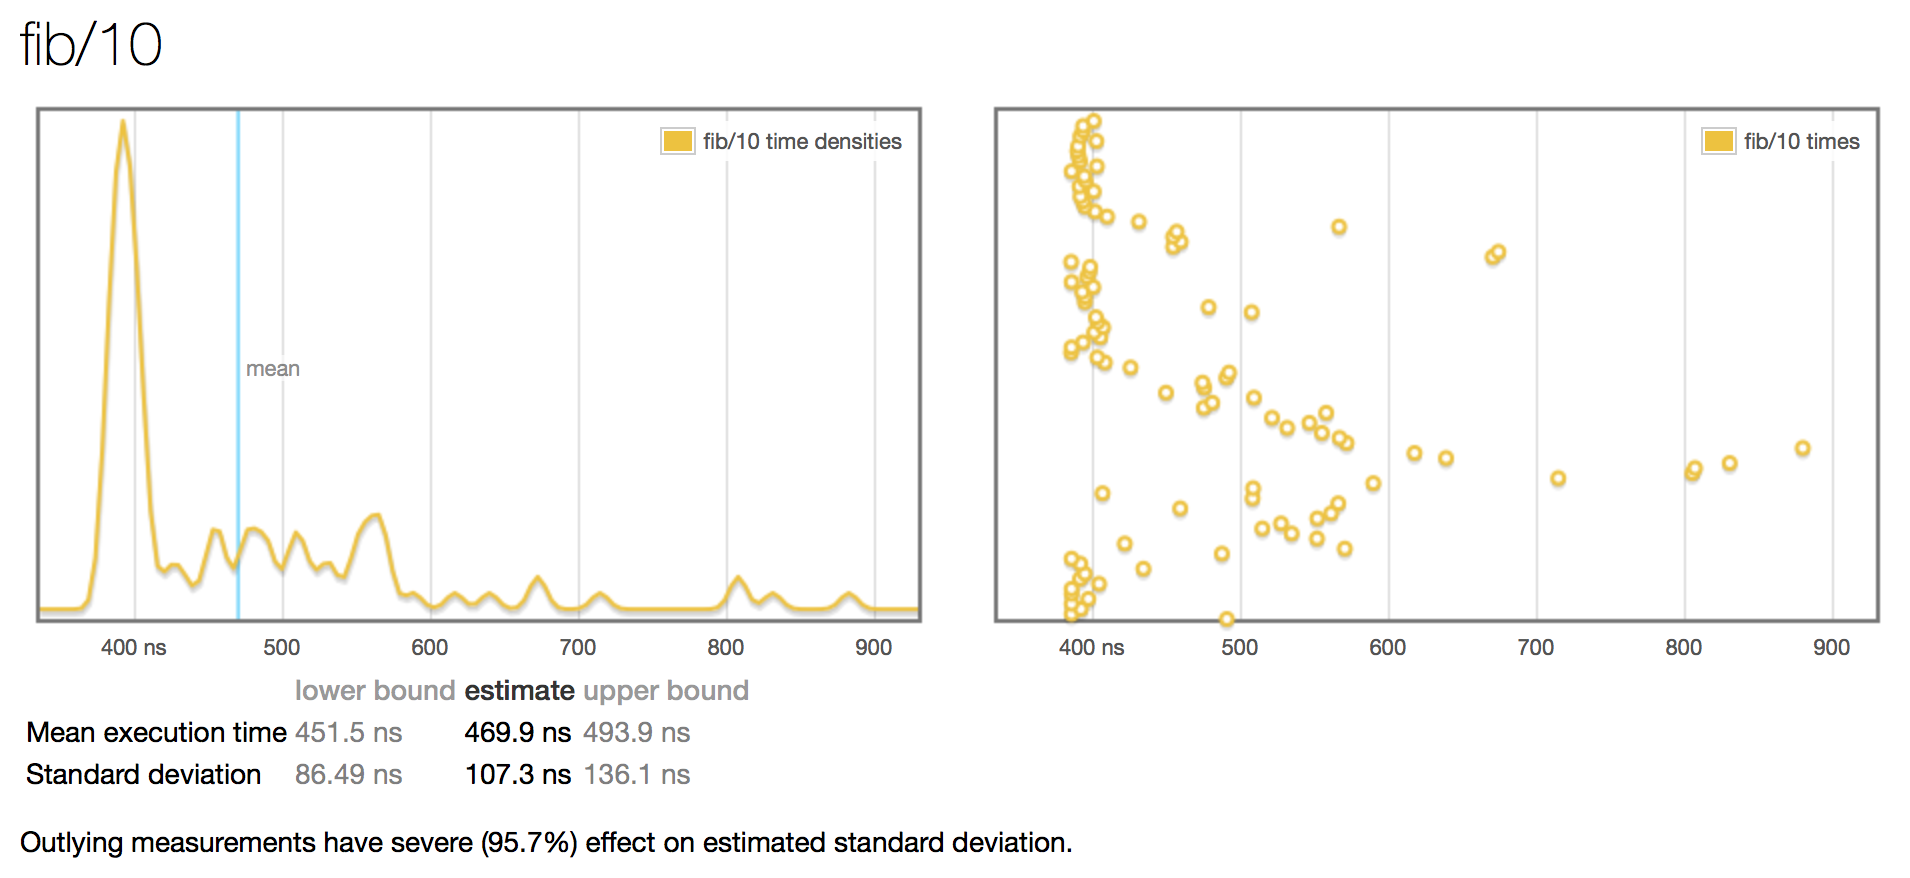
\includegraphics[scale=0.45]{img/criterion.png}
  \caption[Criterion Output]{Output from the benchmarking library Criterion}
  \label{fig:criterion}
\end{figure}


\chapter{Application}
\label{application}

We will now discuss the application of the Mock Object pattern to the
OCaml programming language. In this chapter we will cover some
preliminary techniques, such as dependency injection in OCaml, and the
manual creation of a mock module and expectations. We will move on to
discuss a domain specific language for specifying expectations of a
mock module, and the automatic generation of mock modules from a
module interface.

\section{Preliminary discussion}

\subsection{Dependency injection methods in OCaml}
\label{application:di}

Dependency injection (DI) techniques in object oriented languages
typically focus on lifting hard-coded dependencies into a class's
constructor so that dependencies can be injected at object creation
time. In OCaml things are not much different, except that we will use
language features such as functors and first-class modules for
injecting module dependencies. Complex functionality typically found
in more mature DI frameworks is not necessary for the rest of this
work, and we will not describe their implementation here.

%% \lstinputlisting[
%%     caption={Example of dependency injection techniques in OCaml},
%%     label=code:di,
%%     aboveskip=\baselineskip,
%%   ] {code/application/depinj.ml}

\lstinputlisting[
    caption={Example of basic DI techniques in OCaml},
    label=code:di_basic,
    aboveskip=\baselineskip,
  ] {code/application/depinj_basic_functor.ml}

In listing \ref{code:di_basic} we see a basic DI technique. We
``lift'' the SUT into a functor which receives the DOC. We can use
this method to specialize the SUT with either the ``production'' or
``test'' DOC at compile time.

There are downsides to DI via functorisation, however. In order to
lift the SUT, we have to do significant refactoring -- especially if
the module in question is at the top-level of a compilation unit,
because ml files cannot be functors.

A pattern for lifting a top-level module into a functor is to surround
the whole file with a new module called \code{Make}: \code{module Make
  (D : DOC) = struct ...}, and at the end of the file, after we end
the Make module, add \code{include Make(DOC)}, which will modify this
module so that it contains both a functor to create a new module, and
the original contents of the module. If the ml file is restricted by
an mli file, it may be simpler to just move the functor to a new ml
file (say, ``SUT\_func.ml''), and have the original ml file contain only
the line \code{include SUT_func.Make(DOC)}.

\lstinputlisting[
    caption={Example of DI in OCaml using first-class modules},
    label=code:di_fcm,
    aboveskip=\baselineskip,
] {code/application/depinj_fcm.ml}

Alternatively, instead of using functors, we could use first-class
modules to perform dependency injection. We have a couple different
options at our disposal when using first-class modules. Our first
option is to modify each function in the SUT which depends on the DOC
so that it receives the DOC as a first-class module. This is shown in
function \code{g} of listing \ref{code:di_fcm}. We make this an
optional arguement so that we don't have to modify the callers.

Modifying the parameter list of each of the SUT's functions may not be
practical. Instead, our second option is to create a first-class
module reference, which points to the current DOC. The caller of the
SUT would set this reference before executing the SUT's
functions. Each function must then be modified to reference the DOC
through the first-class module.

These two methods using first-class modules are best used when
modifying existing code for dependency injection, when the SUT being
modified makes use of the DOC in only a few places. If use of the DOC
in the SUT is pervasive, full module lifting may be a better option.

\lstinputlisting[
    caption={Example of a DI ``Factory'' in OCaml},
    label=code:di_factory,
    aboveskip=\baselineskip,
  ] {code/application/depinj_factory.ml}

Another issue with the above first-class module DI technique is that
it pushes the choice of which DOC to use, either the production module
or the test module, down into the caller of the SUT. We may prefer to
make that decision elsewhere, so that neither the SUT nor the SUT's
callers need to know what DOC is being used.

We can acheive this goal with first-class modules using a ``module
factory,'' as in listing \ref{code:di_factory}. This is analogous to a
``factory'' in the object-oriented sense. Client modules would ask
this factory to create a particular module, and the module factory
would check whether it should return the production dependency or the
test dependency, depending on perhaps a command-line flag or some
configuration file. A major benefit to this method is that it removes
the need to refactor each of the functions that access the first class
module, because we can set this module at module initialisation time.

\lstinputlisting[
    caption={Usage of various DI techniques in OCaml},
    label=code:di_useage,
    aboveskip=\baselineskip,
  ] {code/application/depinj_usage.ml}

%% \section{Design considerations for mock modules}
%% \label{application:manual-mock}

\subsection{An example: the simplest mock module implementation}
\label{application:simple}

Before we can automatically generate a mock module from a given
interface, we must first describe how to create manually-written
(hard-coded) mock modules.

Note that this method does not provide any features we would expect
from a full-featured mocking framework such as JMock. There is no
automatic generation of the mock implementation. There is no
expectation language, or even a means to specify expectations. And
because there is no way to specify expectations, the test case must
set up the mocked functions manually, and verify the behaviour of the
SUT manually.

While this is a very simplistic method for creating a mock module, we
will continually extend this method in the following sections, until
we have automatically generated mocks with an expression
language.

Figure \ref{code:mock_real} shows an implementation of a module which
we will mock throughout the next few sections. This module is called
\code{Turtle}, and describes a simple drawing program which is meant
to be reminiscent of the educational programming language
Logo.\footnote{\url{http://en.wikipedia.org/wiki/Logo_(programming_language)}}
We will treat the \code{Turtle} module as our DOC which we wish to
mock.

\lstinputlisting[
caption={An example module that we wish to mock},
label=code:mock_real,
aboveskip=\baselineskip,
] {code/application/simplest_mock_real.ml}

We see from the \code{TURTLE} signature that the \code{Turtle} module
implements a simple interface. There are functions to make a new
turtle, to turn the turtle $90^o$ in either direction, to move the
turtle forward by a given number of units, and to put the pen up or
down. When the pen is in the down position, moving the turtle would
draw to the screen. We have included a simpile combinator operator
\code{>>} which allows us to easily chain together turtle operations.

Figure \ref{code:mock_usage} shows a short program which demonstrates
how one might use the \code{Turtle} library.

\lstinputlisting[
caption={Example usage of the \code{Turtle} library},
label=code:mock_usage,
aboveskip=\baselineskip,
] {code/application/simplest_mock_usage.ml}

Suppose now that we wish to test a function or module which depends
upon this \code{Turtle} library. We may wish to test that this system,
say, calls the \code{turn} function a certain number of times. We can
create a manually mocked implementation of the \code{TURTLE} interface
which replaces the origina \code{turn} function with one which records
the number of function invocations, the arguments of the function
calls, and a pre-set value for the function to return upon
invocation. Figure \ref{code:mock_partial} shows such an
implementation of a partial, manual mock of the \code{Turtle} library.

%% Nodes from simplest_mock_partial.ml:
%%
%% A partial mock of TURTLE (only mock's turn function). This works by
%% including the to-be-mocked module in the mock itself, and
%% reimplementing the functions we want to mock. This won't work if
%% initialising the to-be-mocked module will have unwanted side
%% effects.

\lstinputlisting[
caption={A manually mocked OCaml module},
label=code:mock_partial,
aboveskip=\baselineskip,
] {code/application/simplest_mock_partial.ml}

We can use this partial mock by installing it using any of the
dependency injection techniques described section
\ref{application:di}, and then write our test using the newly mocked
DOC. Manually mocking a module in this way might be an effective way
to write a test that would otherwise be impossible, but manually
mocking modules in this manner is tedius and cumbersome. We would much
prefer a method which allows us to describe the way that we expect the
depended upon component to behave when it is interacting with the test
case, and then generate a mock module from that set of expectations.

%\section{Specifying a mock's expectations}
\section{Implementation of the mocking framework}
\label{application:implementation}

%% Synopsis

Much of the Mock Pattern's power comes from having a lightweight
expectation specification language. This language allows users to
describe their expectations of how the mock module will behave in a
``natural'' way. Expectations are then ``compiled'' into the
underlying data type representation. The mock module, while being
exercised by the system under test, records its interactions and also
plays back the indirect outputs recorded in the expectations. Finally,
the expectations are verified by the test framework by checking that
the recorded interactions with the mocked module match what was
specified by the user in the expectations.

\subsection{Syntax of the expression language}
\label{application:syntax}

\textit{Much of the Mock Pattern's power comes from having a
  lightweight expectation specification DSL. In this section we
  describe the design and implementation of an expectation DSL in
  OCaml which is similar to the JMock expectation DSL described in
  section \ref{testdoubles:mocks}.}

\textit{Some considerations when implementing
  expectations. Expectations are used for two purposes: 1) to allow
  the mock implmentation to provide the appropriate indirect inputs to
  the SUT (through the expectation's actions), and 2) to provide
  indirect outputs to the test case from the SUT, in the form of
  invocation counts, as well as values passed to the mocked
  functions.}

\textit{For expectations, we need to keep track of the expected
  invocation count, and the expected outputs of the function, whether
  they are values or expections. When (and if) we implement individual
  sequences, we need to keep track of which expectations are in which
  sequence.}

\textit{While running the test case, the mock implementation needs to
  keep track of the invocations of each function, including the order
  in which they were called, as well as with what arguments they were
  called.}

\textit{Note: a feature that we'd like to have is expectation pattern
  matching. We'd like to be able to set an expectation that a function
  will be called with some pattern-restricted set of arguments, and
  then either verify that the the function was invoked with arguments
  that match the pattern, or simply inspect the arguements passed to
  the function in the test itself. We might want to implement this
  feature by allowing the user to pass arbitrary funtions which match
  the type of the mocked function to the mock as the mock function
  itself, instead of generating an entire function using just the
  invocation arguments and expected return value.}

%% \subsection{Implementation of mock module implementing the expression langauge}
\subsection{Verifying the expression language}
\label{application:mock_impl}

\subsubsection{Module organisation}

We will be generating a lot of code when we generate mock
modules. We'll have to generate an implementation of the to-be-mocked
interface. We'll have to generate expectation language code which uses
the same types as defined in the to-be-mocked interface, such that
the types in the expectation langauge will unify with those in the
mocked module. We'll have to generate code to verify the expectations
that have been defined in the test case.

The organisation of generated modules must be chosen carfully,
especially to satisfy the requirement that types between the
expectation langauge and the mocked module must unify.

One solution to this is to put logically separate code into separate
modules, and strategically include modules in ``derivative'' modules
where necessary. (This is what we have currently done.) Doing this
allows us to properly namespace the identifiers that we have
generated, so that we don't have to mangle generated names and then
redefine them later.

Another solution is to place all generated code into a single module
that is not exported, but to then create separate modules (say
\code{E} for the expecation language and \code{M} for the mocked
module), where each of these modules is restriced by an appropriate
signature. This should give us the most flexibility: no cumbersome
module inclusions, while hopefully retaining types that are
unifiable. Unfortunately, with this solution we will have to mangle
our generated names and then redefine them later, because we may clash
with the names in our to-be-mocked interface. We can minimise the
names we have to mangle by keeping track of the identifiers defined in
the to-be-mocked module, and only mangling clashing names. On second
thought, this sounds far too complex; more complex than managing
multiple modules.

\subsubsection{Generalised Algebraic Data Types}
\label{application:gadt}

We make use of Generalised Algebraic Data Types (GADTs) to help us
encode the arguements for and return values of our expectations. GADTs
are a relatively new feature in OCaml. They allow \dots

% (Also cite Ralf's Phantom Types paper! :) )

\subsubsection{Verifying expectations}

To verify expectations, we need to compare them to the invocation
record, and ensure that the invocations satisfy the expecatations. We
need to ensure:

\begin{enumerate}
\item All invocation counts are satisfied. This includes insuring that
  \textit{never} functions are not called, and that number-checked
  functions are called the correct number of times. We can skip
  testing for \textit{allowing} functions, since we don't care whether
  they are called.
\item Sequenced expectations are invoked in the order
  specified. (We'll do this later, not as a first feature.)
\end{enumerate}

To verify expectations, we need to iterate over each invocation, and
imperatively update the list of expectations accordingly. We search
for the current invocation in the list of expectations, and increment
the invocation count. After we've interated through the invocations,
we have an updated list of expectations that we can then verify
(short-cut: we update the list of expectations at test-time, instead
of recording invocations). Now we proceed through the expectations and
verify that the invocation count satisfies the expectation. Later,
when we implement sequences, we can also verify that the order of
invocations is correct.\footnote{Aha! We can simply attach an
  invocation sequence number to each expectation as we invock a
  matching function. This will allow us to verify that the
  expectations in each sequence have a monotonically increasing
  invocation sequence number.}

We should be sure to proceed through the entire list of expectations,
and not necessarily short-circuit at the first matching
expectation. If that first matching expectation has already been
satisfied, then we will need to proceed to the next potentially
matching expectation. This means that we will need to perform
verification at each invocation step, so that we can easily skip
already-satisifed expectations.

\subsection{Automatic generation of a mock module}
%% \section{Automatically generating mock modules}
\label{application:generation}

Mocks are only truly useful as a testing tool when they can be
automatically generated from an interface. We will use Camlp4, an
OCaml preprocessing tool, a new OCaml feature called \textit{extension
  points} used for AST annotation, and the OCaml compiler's
\textit{compiler-libs} in order to generate and pretty-print OCaml
code.

\chapter{Reflection}
\label{reflection}

\section{Reflect}



%% Bibliography
%\nocite{*}
\bibliographystyle{plain}
\bibliography{bibliography}

\end{document}
